% Options for packages loaded elsewhere
\PassOptionsToPackage{unicode}{hyperref}
\PassOptionsToPackage{hyphens}{url}
\PassOptionsToPackage{dvipsnames,svgnames*,x11names*}{xcolor}
%
\documentclass[
  10pt,
  ignorenonframetext,
  aspectratio=43,
]{beamer}
\usepackage{pgfpages}
\setbeamertemplate{caption}[numbered]
\setbeamertemplate{caption label separator}{: }
\setbeamercolor{caption name}{fg=normal text.fg}
\beamertemplatenavigationsymbolsempty

%%
%%% Definition of colors
%%% Source: https://latexcolor.com/
\definecolor{blanchedalmond}{rgb}{1.0, 0.92, 0.8}
\definecolor{blond}{rgb}{0.98, 0.94, 0.75}
%%% End of definition of colors
%%

% Prevent slide breaks in the middle of a paragraph
\widowpenalties 1 10000
\raggedbottom
\usepackage{lmodern}
\usepackage{amssymb,amsmath}
\usepackage{ifxetex,ifluatex}
\ifnum 0\ifxetex 1\fi\ifluatex 1\fi=0 % if pdftex
  \usepackage[T1]{fontenc}
  \usepackage[utf8]{inputenc}
  \usepackage{textcomp} % provide euro and other symbols
\else % if luatex or xetex
  \usepackage{unicode-math}
  \defaultfontfeatures{Scale=MatchLowercase}
  \defaultfontfeatures[\rmfamily]{Ligatures=TeX,Scale=1}
  \setmainfont[]{Myriad Pro}
  \ifxetex
    \usepackage{xeCJK}
    \setCJKmainfont[ItalicFont=AR PL UKai TW]{AR UDJingXiHeiPU30}
  \fi
  \ifluatex
    \usepackage[]{luatexja-fontspec}
    \setmainjfont[ItalicFont=AR PL UKai TW]{AR UDJingXiHeiPU30}
  \fi
\fi
\usetheme[]{metropolis}
\usecolortheme{default}
\usefonttheme{serif} % use mainfont rather than sansfont for slide text
% Use upquote if available, for straight quotes in verbatim environments
\IfFileExists{upquote.sty}{\usepackage{upquote}}{}
\IfFileExists{microtype.sty}{% use microtype if available
  \usepackage[]{microtype}
  \UseMicrotypeSet[protrusion]{basicmath} % disable protrusion for tt fonts
}{}
\makeatletter
\@ifundefined{KOMAClassName}{% if non-KOMA class
  \IfFileExists{parskip.sty}{%
    \usepackage{parskip}
  }{% else
    \setlength{\parindent}{0pt}
    \setlength{\parskip}{6pt plus 2pt minus 1pt}}
}{% if KOMA class
  \KOMAoptions{parskip=half}}
\makeatother
\usepackage{xcolor}
\IfFileExists{xurl.sty}{\usepackage{xurl}}{} % add URL line breaks if available
\IfFileExists{bookmark.sty}{\usepackage{bookmark}}{\usepackage{hyperref}}
\hypersetup{
  pdftitle={Reserving Female Status --- Women Reserved Seats and Gender Empowerment in Taiwan},
  pdfauthor={何雨忻},
  colorlinks=true,
  linkcolor=Maroon,
  filecolor=Maroon,
  citecolor=Blue,
  urlcolor=red,
  pdfcreator={LaTeX via pandoc}}
\urlstyle{same} % disable monospaced font for URLs
\newif\ifbibliography
\usepackage{listings}
\newcommand{\passthrough}[1]{#1}
\lstset{defaultdialect=sh}
\lstset{framexleftmargin=0mm, frame=trBL,backgroundcolor=\color{blanchedalmond!5},numbers=left,numberstyle=\scriptsize,basicstyle=\small}
\lstset{aboveskip=5mm,belowskip=5mm,xleftmargin=20pt,xrightmargin=5pt}
% \lstset{prebreak={\raisebox{0ex}[0ex][0ex]}}
% \lstset{postbreak={\raisebox{0ex}[0ex][0ex]\space}}
\lstset{breaklines=true,breakatwhitespace=true}
\usepackage{longtable,booktabs}
\usepackage{caption}
% Make caption package work with longtable
\makeatletter
\def\fnum@table{\tablename~\thetable}
\makeatother
\usepackage{graphicx,grffile}
\makeatletter
\def\maxwidth{\ifdim\Gin@nat@width>\linewidth\linewidth\else\Gin@nat@width\fi}
\def\maxheight{\ifdim\Gin@nat@height>\textheight\textheight\else\Gin@nat@height\fi}
\makeatother
% Scale images if necessary, so that they will not overflow the page
% margins by default, and it is still possible to overwrite the defaults
% using explicit options in \includegraphics[width, height, ...]{}
\setkeys{Gin}{width=\maxwidth,height=\maxheight,keepaspectratio}
% Set default figure placement to htbp
\makeatletter
\def\fps@figure{htbp}
\makeatother
\setlength{\emergencystretch}{3em} % prevent overfull lines
\providecommand{\tightlist}{%
  \setlength{\itemsep}{0pt}\setlength{\parskip}{0pt}}
\setcounter{secnumdepth}{-\maxdimen} % remove section numbering

%
% When using babel or polyglossia with biblatex, loading csquotes is recommended 
% to ensure that quoted texts are typeset according to the rules of your main language.
%
\usepackage{csquotes}

%
% blockquote
%
\definecolor{blockquote-border}{RGB}{221,221,221}
\definecolor{blockquote-text}{RGB}{89,89,89}
\usepackage{mdframed}
\newmdenv[rightline=false,bottomline=false,topline=false,linewidth=3pt,linecolor=blockquote-border,skipabove=\parskip]{customblockquote}
\renewenvironment{quote}{\begin{customblockquote}\list{}{\rightmargin=0em\leftmargin=0em}%
\item\relax\color{blockquote-text}\ignorespaces}{\unskip\unskip\endlist\end{customblockquote}}

%
% Source Sans Pro as the de­fault font fam­ily
% Source Code Pro for monospace text
%
% 'default' option sets the default 
% font family to Source Sans Pro, not \sfdefault.
%

\usepackage{tikz}
\usepackage{pgfplots}
\usepackage{adjustbox}
\usepackage{booktabs}
\linespread{1.3}
\usepackage[font={footnotesize}]{caption}

\title{Reserving Female Status --- Women Reserved Seats and Gender
Empowerment in Taiwan}
\subtitle{Applied Microeconomics, 2022 Spring}
\author{何雨忻}
\date{Apr 25, 2022}
\institute{Department of Economics, National Taiwan University}

\begin{document}
\frame{\titlepage}

\begin{frame}{Policy Background}
\protect\hypertarget{policy-background}{}
Mandatory women reserved seats was codified in \emph{ROC Constitution}
since 1946

\begin{itemize}
\tightlist
\item
  Long before western feminism movement in 1960s
\item
  Mainly Influenced by May Fourth Movement(新文化運動)and KMT-CCP
  Alliance(聯俄容共)(黃長玲,2012)
\end{itemize}

\begin{block}{Women in politics}
\protect\hypertarget{women-in-politics}{}
Women parliamentarians (from CEC, OECD database)

\begin{longtable}[]{@{}cccccc@{}}
\toprule
Taiwan & Korea & Japan & Singapore & Denmark & Sweden \\
\midrule
\endhead
41.6\% & 19\% & 9.9\% & 23\% & 39.7\% & 47\% \\
\bottomrule
\end{longtable}
\end{block}
\end{frame}

\begin{frame}{Empirical Literatures in India}
\protect\hypertarget{empirical-literatures-in-india}{}
\begin{itemize}
\tightlist
\item
  1993 Constitutional Amendment
\item
  Outcomes:

  \begin{itemize}
  \tightlist
  \item
    Increased female political representation
  \item
    Female entrepreneurship \footnotesize (Ghani, Kerr, and O'Connell
    2014) \normalsize
  \item
    Report of crimes against women \footnotesize (Iyer et al.~2012)
    \normalsize
  \item
    Neonatal mortality of female \footnotesize (Kalsi 2017) \normalsize
  \item
    Female educational attainment \footnotesize (Beaman et al.~2012)
    \normalsize
  \end{itemize}
\end{itemize}
\end{frame}

\begin{frame}{Data \& Empirical Strategy}
\protect\hypertarget{data-empirical-strategy}{}
\begin{block}{Outcomes}
\protect\hypertarget{outcomes}{}
\begin{itemize}
\tightlist
\item
  Son preference

  \begin{itemize}
  \tightlist
  \item
    Willingness to have 3rd parity (MOI birth data, 1999 --- 2006)
  \item
    Gender difference of neonatal mortality rate
  \end{itemize}
\item
  Gender role attitude (Taiwan Social Change Survey, 2006, 2011, 2016)
\end{itemize}

\begin{figure}
\centering
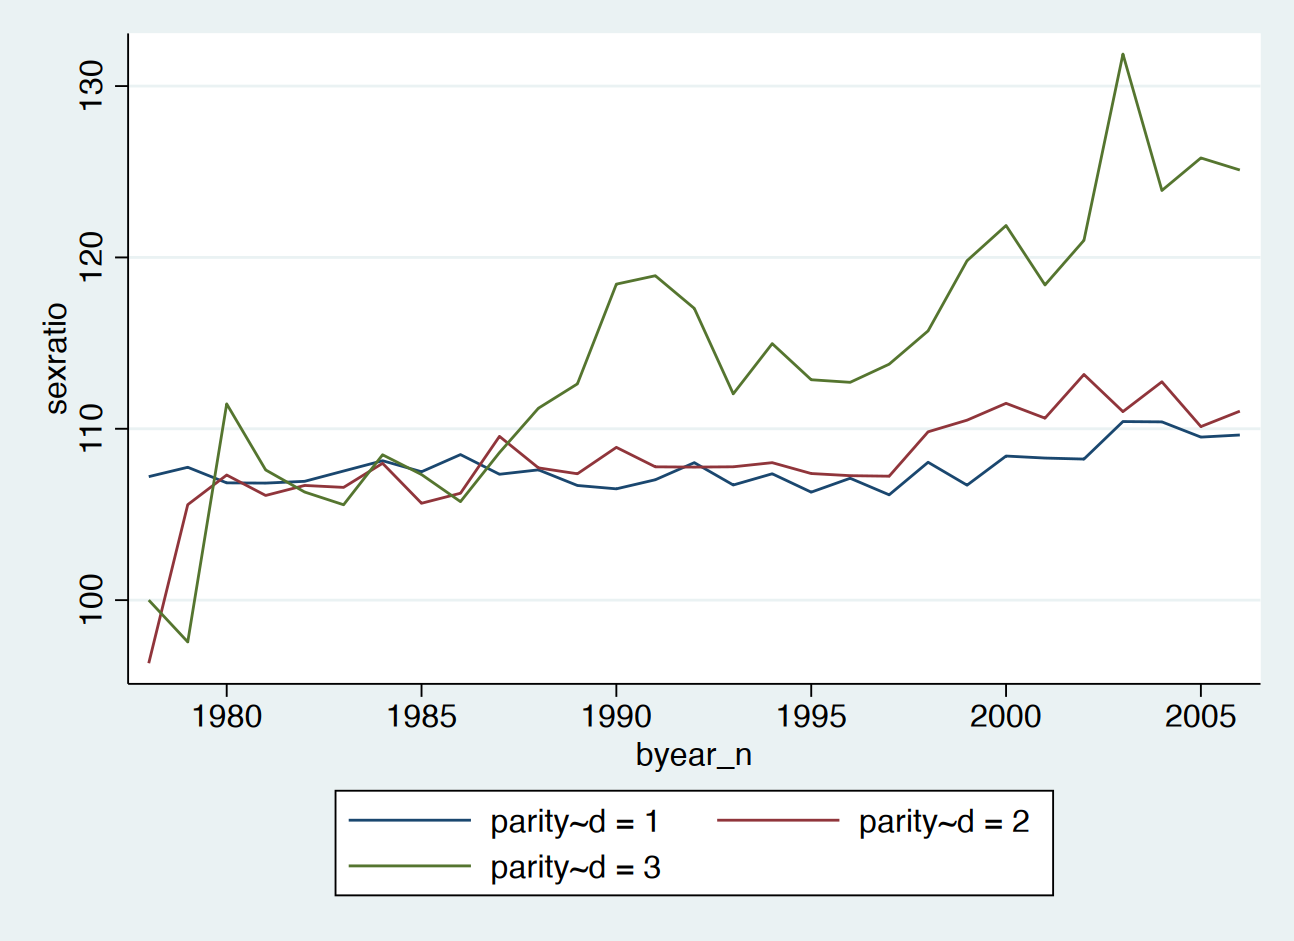
\includegraphics[width=0.6\textwidth,height=\textheight]{20220425-applied-micro-women-reserved-seats-proposal.assets/sexratioByParity.png}
\caption{Newborn Sex Ratio by Parity}
\end{figure}
\end{block}
\end{frame}

\begin{frame}
\begin{block}{Treatment}
\protect\hypertarget{treatment}{}
Council member elections, 1999 --- 2006

\begin{itemize}
\tightlist
\item
  Endogenous treatment \(X\): \textbf{Proportion of female council
  member}
\item
  Instrument \(Z\): \textbf{Proportion of reserved seats}
\item
  Control for population to prevent OVB in the first stage.
\end{itemize}

\begin{figure}[htb]
\centering
\scalebox{0.6}{
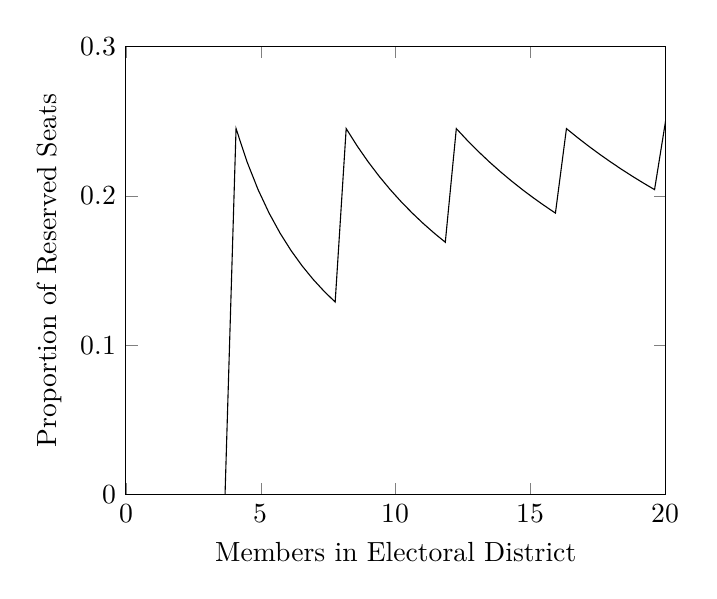
\begin{tikzpicture}
\begin{axis}
[
    xlabel={Members in Electoral District}, 
    ylabel={Proportion of Reserved Seats}, 
    xmin=0, 
    xmax=20, 
    ymin=0, 
    ymax=0.3
]
\addplot[no marks, domain=0:20, samples=50] {floor(x/4)/x};
\end{axis}
\end{tikzpicture}
}
\caption{Discontinuity of Reserved Seats by Policy Design}
\end{figure}
\end{block}
\end{frame}

\begin{frame}{Contribution}
\protect\hypertarget{contribution}{}
\begin{itemize}
\tightlist
\item
  Casual effect of political participation on gender empowerment, with
  neater identification.
\item
  Potential channels of changing gender attitudes.
\end{itemize}
\end{frame}

\end{document}
